\documentclass[a4paper,10pt]{article}
   \usepackage[english]{babel}
   \usepackage{blindtext}
   \usepackage[T1]{fontenc}
   \usepackage{comment}
   \usepackage{graphicx}
   \begin{document}

   \begin{section}{Introduction to GemaTreeAC 2=0}
     GemaTreeAC 2=0 is a gematria calculator, numerological classification algorithm and a database.
     Gematria is the mapping of alphabetical characters to numbers by a cipher. The mapping is represented by
     key-value pairs, the key being the letter and value the number. An ordinal cipher would map a to 1, b to 2,
     c to 3 and so on. Words have gematria values, too, according to the cipher. The characters in a word are mapped to
     numbers and their sum is the gematria value of a word. If two words have the same gematria value,
     they are regarded as as semantically related.

     GemaTreeAC has a few more relations than that of the identical gematria value.
     Numerological reduction creates new categories for numbers:
     These are the n-digit set, the root number and the
     route from leaf to root of a number. GeamTreeAC uses this data
     to compete numeral pairs by their numerological properties.
     Gematria value of a word is denoted here by $v$
     
     \[
     \forall v, v \in N_0
     \]


     The plot also uses simple distance measures:
     \[d_{property_{v_0,v_1}} = |property_{v_0} - property_{v_1}|\] The distances from
     this process are plotted in a scatter diagram and
     different numerological relations are color coded. In the following formulas, $v_0$
     is the searched for gematria value of a word and $v_1$ is a gematria value of a word found in the database.

     The numerological distance is calculated as
     \[
     \delta_{v_0, v_1} = \frac{  d_{nds_{v_0,v_1}}+d_{root_{v_0,v_1}}+d_{gematria_{v_0,v_1}}  }
     {  points_{nds} + points_{root} + points_{route} + points_{gematria} + points_{word}  }
     \] with some biases and weights to better control the distance measure search results and the plot.

     GemaTreeAC's algorithm uses distance measure $\delta$ and an angle $\phi$ to calculate the coordinates of a number.
     The angle is expressed as
     \[
     \phi = \frac{v}{v_{max}}*360^\circ \textrm{where $v_{max}$ is the highest $v$ in current search} 
     \]

     In the plot,
     \[
     x = sin\phi*\delta \quad \textrm{and} \quad y = cos\phi*\delta
     \]

     The length of a number means the number of digits in a value here.

     \[
     length_v = \textrm{ number of digits in } v.
     \]

     The n-digit set of $v$ is defined as
     \[
     \nu_v = [10^{length_v-1}, ... , 9*(10^0 + 10^1 + 10^2 +, ..., + 10^{length_v-1})]
     \]

     It is true that
     \[
     \forall v, v \in \nu_{length_v}
     \]

     Numerological reduction is calculated as
     \[
     parent_v = \sum_{n=0}^{n=length_v}v_n
     \]

     The root number is reached when
     \[
     v \in \nu_1
     \]

     The route to root is defined as
     \[
     route_v = [v, f(v)=f(parent_v)]
     \]

     This means that number $666$ has the route $[666, 18, 9]$ and $123$ has the route $[123, 6]$.
     
   \end{section}

   \begin{section}{The DMS Plot}

     \begin{figure}
       \centering
       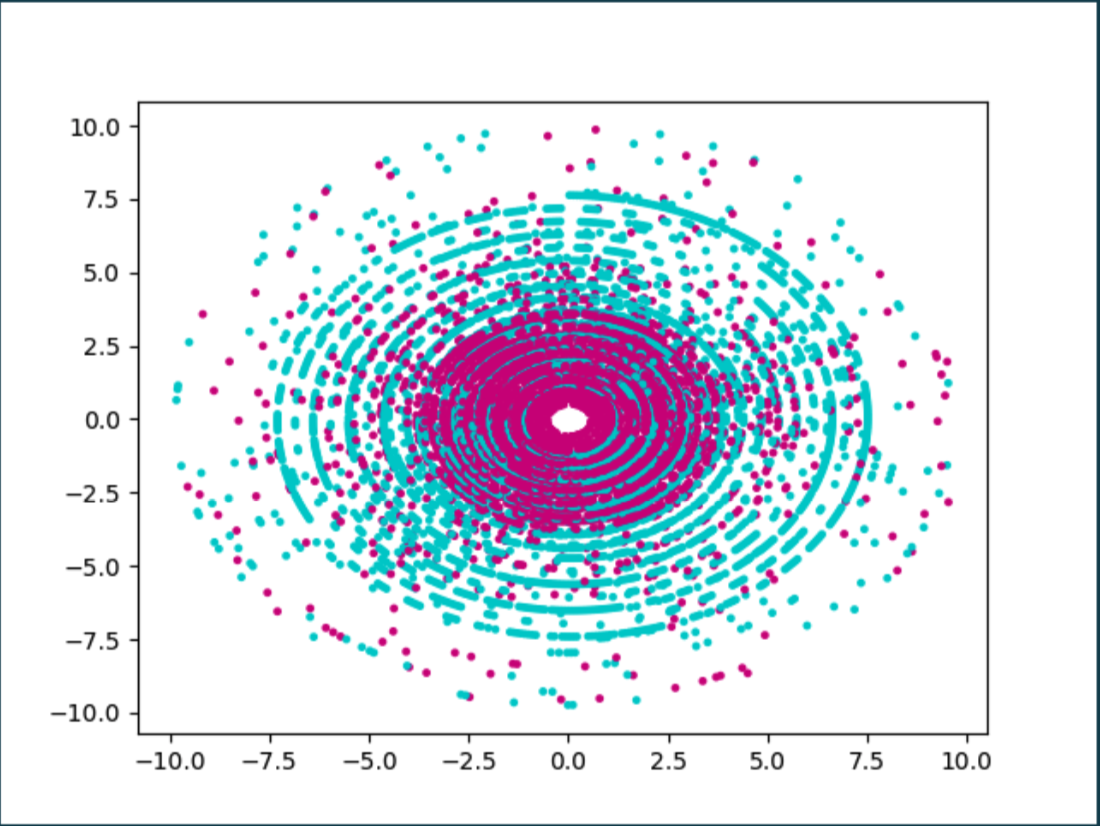
\includegraphics[width = 240px, height = 180px]{suuripetotaivos66360}
       \caption{DMS Plot of word 'suuripetotaivos', gematria 66360 in Fibonacci cipher.}
     \end{figure}

     \begin{figure}
       \centering
       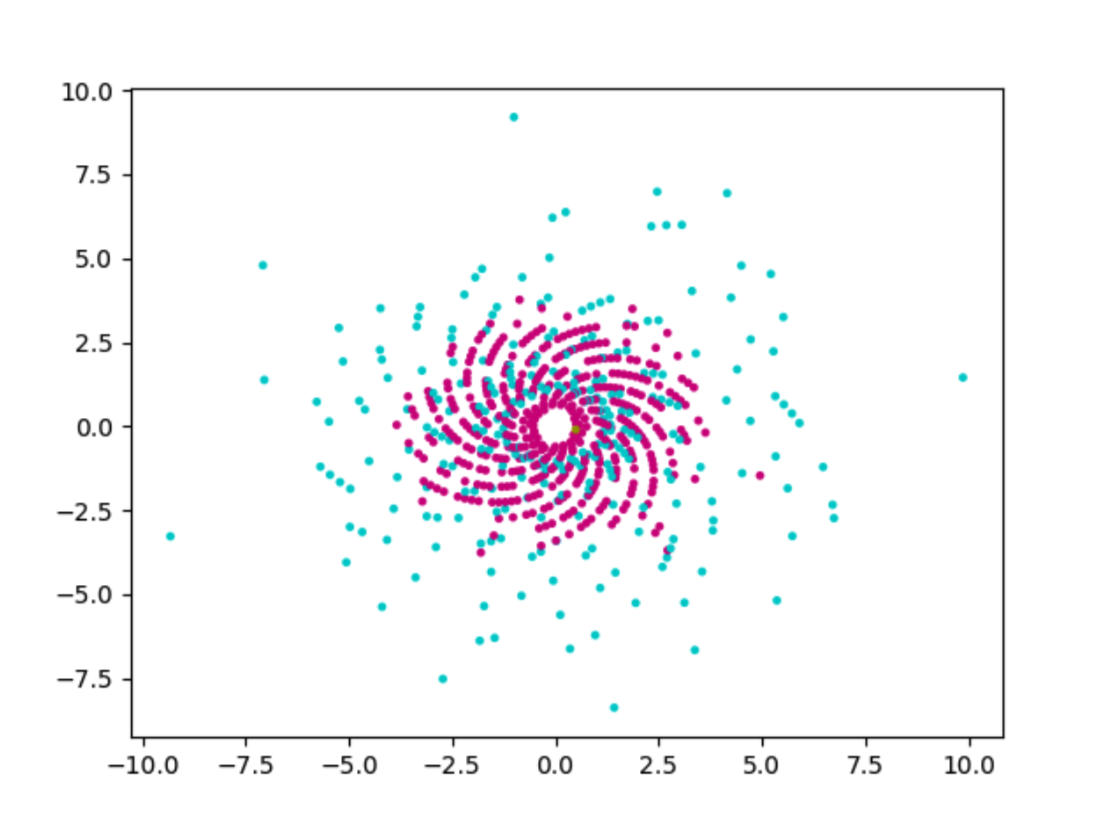
\includegraphics[width = 240px, height = 180px]{komplicerande387}
       \caption{DMS Plot of word 'komplicerande', gematria 387 in English Extended cipher.}
     \end{figure}

     \begin{figure}
       \centering
       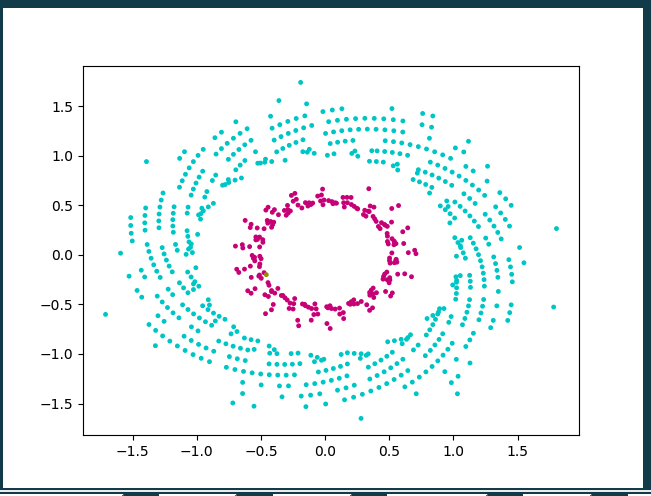
\includegraphics[width = 240px, height = 180px]{suuripeto1134}
       \caption{DMS Plot of word 'suuripeto', gematria 1134 in English Extended cipher.}
     \end{figure}
     
   \end{section}
   

   \end{document}

   
